%% LyX 2.2.1 created this file.  For more info, see http://www.lyx.org/.
%% Do not edit unless you really know what you are doing.
\documentclass[10pt]{beamer}\usepackage[]{graphicx}\usepackage[]{color}
%% maxwidth is the original width if it is less than linewidth
%% otherwise use linewidth (to make sure the graphics do not exceed the margin)
\makeatletter
\def\maxwidth{ %
  \ifdim\Gin@nat@width>\linewidth
    \linewidth
  \else
    \Gin@nat@width
  \fi
}
\makeatother

\definecolor{fgcolor}{rgb}{0.345, 0.345, 0.345}
\newcommand{\hlnum}[1]{\textcolor[rgb]{0.686,0.059,0.569}{#1}}%
\newcommand{\hlstr}[1]{\textcolor[rgb]{0.192,0.494,0.8}{#1}}%
\newcommand{\hlcom}[1]{\textcolor[rgb]{0.678,0.584,0.686}{\textit{#1}}}%
\newcommand{\hlopt}[1]{\textcolor[rgb]{0,0,0}{#1}}%
\newcommand{\hlstd}[1]{\textcolor[rgb]{0.345,0.345,0.345}{#1}}%
\newcommand{\hlkwa}[1]{\textcolor[rgb]{0.161,0.373,0.58}{\textbf{#1}}}%
\newcommand{\hlkwb}[1]{\textcolor[rgb]{0.69,0.353,0.396}{#1}}%
\newcommand{\hlkwc}[1]{\textcolor[rgb]{0.333,0.667,0.333}{#1}}%
\newcommand{\hlkwd}[1]{\textcolor[rgb]{0.737,0.353,0.396}{\textbf{#1}}}%
\let\hlipl\hlkwb

\usepackage{framed}
\makeatletter
\newenvironment{kframe}{%
 \def\at@end@of@kframe{}%
 \ifinner\ifhmode%
  \def\at@end@of@kframe{\end{minipage}}%
  \begin{minipage}{\columnwidth}%
 \fi\fi%
 \def\FrameCommand##1{\hskip\@totalleftmargin \hskip-\fboxsep
 \colorbox{shadecolor}{##1}\hskip-\fboxsep
     % There is no \\@totalrightmargin, so:
     \hskip-\linewidth \hskip-\@totalleftmargin \hskip\columnwidth}%
 \MakeFramed {\advance\hsize-\width
   \@totalleftmargin\z@ \linewidth\hsize
   \@setminipage}}%
 {\par\unskip\endMakeFramed%
 \at@end@of@kframe}
\makeatother

\definecolor{shadecolor}{rgb}{.97, .97, .97}
\definecolor{messagecolor}{rgb}{0, 0, 0}
\definecolor{warningcolor}{rgb}{1, 0, 1}
\definecolor{errorcolor}{rgb}{1, 0, 0}
\newenvironment{knitrout}{}{} % an empty environment to be redefined in TeX

\usepackage{alltt}
\usepackage[T1]{fontenc}
\setcounter{secnumdepth}{3}
\setcounter{tocdepth}{3}
\usepackage{url}
\ifx\hypersetup\undefined
  \AtBeginDocument{%
    \hypersetup{unicode=true,pdfusetitle,
 bookmarks=true,bookmarksnumbered=false,bookmarksopen=false,
 breaklinks=false,pdfborder={0 0 0},pdfborderstyle={},backref=false,colorlinks=false}
  }
\else
  \hypersetup{unicode=true,pdfusetitle,
 bookmarks=true,bookmarksnumbered=false,bookmarksopen=false,
 breaklinks=false,pdfborder={0 0 0},pdfborderstyle={},backref=false,colorlinks=false}
\fi
\usepackage{breakurl}

\makeatletter

%%%%%%%%%%%%%%%%%%%%%%%%%%%%%% LyX specific LaTeX commands.
\providecommand{\LyX}{\texorpdfstring%
  {L\kern-.1667em\lower.25em\hbox{Y}\kern-.125emX\@}
  {LyX}}

%%%%%%%%%%%%%%%%%%%%%%%%%%%%%% Textclass specific LaTeX commands.
 % this default might be overridden by plain title style
 \newcommand\makebeamertitle{\frame{\maketitle}}%
 % (ERT) argument for the TOC
 \AtBeginDocument{%
   \let\origtableofcontents=\tableofcontents
   \def\tableofcontents{\@ifnextchar[{\origtableofcontents}{\gobbletableofcontents}}
   \def\gobbletableofcontents#1{\origtableofcontents}
 }

%%%%%%%%%%%%%%%%%%%%%%%%%%%%%% User specified LaTeX commands.
\usetheme{PaloAlto}

\makeatother
\IfFileExists{upquote.sty}{\usepackage{upquote}}{}
\begin{document}


\title[knitr, Beamer, and FragileFrame]{A Minimal Demo of knitr with Beamer and Fragile Frames}

\author{Yihui Xie\thanks{I thank Richard E. Goldberg for providing this demo.}}
\makebeamertitle
\begin{frame}{Background}

\begin{itemize}
\item The \textbf{knitr}\textbf{\emph{ }}package allows you to embed R code
and figures in \LaTeX{} documents

\begin{itemize}
\item It has functionality similar to Sweave but looks nicer and gives you
more control
\end{itemize}
\item If you already have Sweave working in \LyX{}, getting \textbf{knitr}
to work is trivial

\begin{enumerate}
\item Install the \textbf{knitr} package in \emph{R}
\item Read \url{https://yihui.name/knitr/demo/lyx/}
\end{enumerate}
\item If you use Sweave or \textbf{knitr} with Beamer in \LyX{}, you must
use the\emph{ FragileFrame} environment for the frames that contain
R code chunks. Let's see if \textbf{knitr} works with Beamer in this
small demo. 
\end{itemize}
\end{frame}

\section{First Test}
\begin{frame}[fragile]{First Test}

OK, let's get started with just some text:



\begin{knitrout}\footnotesize
\definecolor{shadecolor}{rgb}{0.969, 0.969, 0.969}\color{fgcolor}\begin{kframe}
\begin{alltt}
\hlcom{# create some random numbers}
\hlstd{(x}\hlkwb{=}\hlkwd{rnorm}\hlstd{(}\hlnum{20}\hlstd{))}
\end{alltt}
\begin{verbatim}
##  [1]  0.1449583  0.4383221  0.1531912  1.0849426  1.9995449
##  [6] -0.8118832  0.1602680  0.5858923  0.3600880 -0.0253084
## [11]  0.1508809  0.1100824  1.3596812 -0.3269946 -0.7163819
## [16]  1.8097690  0.5084011 -0.5274603  0.1327188 -0.1559430
\end{verbatim}
\begin{alltt}
\hlkwd{mean}\hlstd{(x);}\hlkwd{var}\hlstd{(x)}
\end{alltt}
\begin{verbatim}
## [1] 0.3217385
## [1] 0.5714534
\end{verbatim}
\end{kframe}
\end{knitrout}

BTW, the first element of \texttt{x} is 0.1449583. (Did you notice
the use of\texttt{ \textbackslash{}Sexpr\{\}}?)
\end{frame}

\section{Second Test}
\begin{frame}[fragile]{Second Test}

Text is nice but let's see what happens if we make a couple of plots
in our chunk:

\begin{knitrout}\footnotesize
\definecolor{shadecolor}{rgb}{0.969, 0.969, 0.969}\color{fgcolor}\begin{kframe}
\begin{alltt}
\hlkwd{par}\hlstd{(}\hlkwc{las}\hlstd{=}\hlnum{1}\hlstd{,}\hlkwc{mar}\hlstd{=}\hlkwd{c}\hlstd{(}\hlnum{4}\hlstd{,}\hlnum{4}\hlstd{,}\hlnum{.1}\hlstd{,}\hlnum{.1}\hlstd{))}  \hlcom{# tick labels direction}
\hlkwd{boxplot}\hlstd{(x)}
\hlkwd{hist}\hlstd{(x,}\hlkwc{main}\hlstd{=}\hlstr{''}\hlstd{,}\hlkwc{col}\hlstd{=}\hlstr{"blue"}\hlstd{,}\hlkwc{probability}\hlstd{=}\hlnum{TRUE}\hlstd{)}
\hlkwd{lines}\hlstd{(}\hlkwd{density}\hlstd{(x),}\hlkwc{col}\hlstd{=}\hlstr{"red"}\hlstd{)}
\end{alltt}
\end{kframe}

{\centering 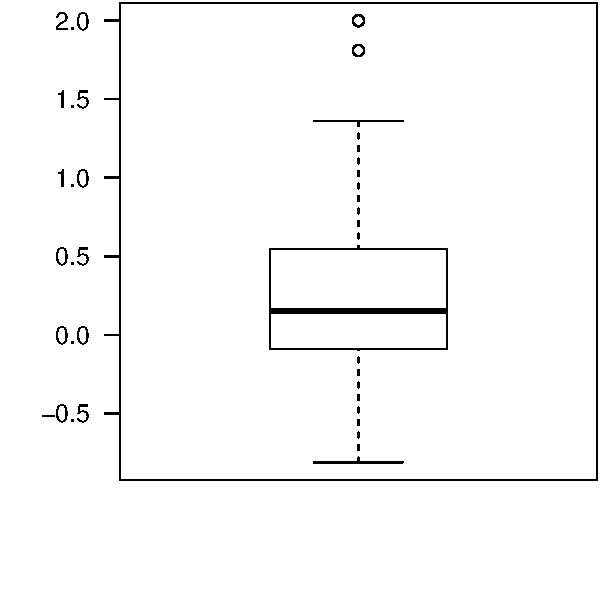
\includegraphics[width=.45\linewidth]{figure/beamer-boring-plots-1} 
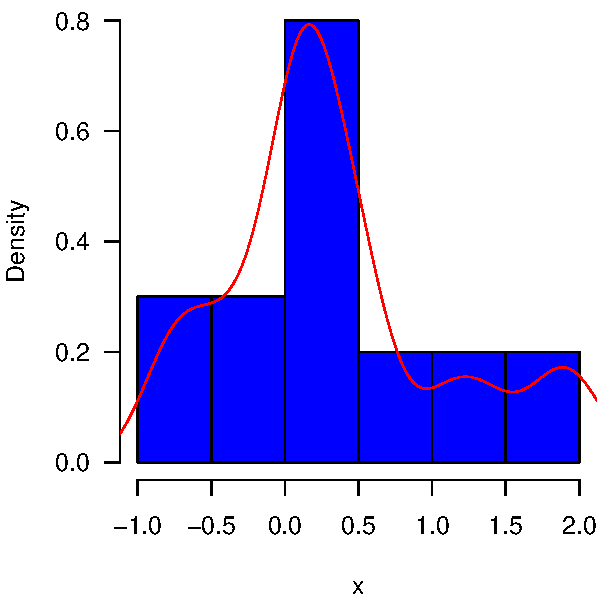
\includegraphics[width=.45\linewidth]{figure/beamer-boring-plots-2} 

}



\end{knitrout}
\end{frame}

\section{The Big Question}
\begin{frame}{The Big Question}

Do the above chunks work? You should be able to compile the \LyX{}
document and get a nice-looking PDF slide presentation. If not, time
to double-check everything...
\end{frame}

\end{document}
